\section*{Detecting Sinusoids}

Before we attempt to transform a time domain signal to the frequency domain, we will need to solve
a simpler problem.  Let us first try and develop a tool to detect whether a particular frequency or
sinusoid is present in some sequence of audio samples.  If we can do that, we can test our samples against
a whole range of frequencies, allowing us to construct a good sketch of the frequency domain of
the sound.  In essence, this is what the DFT does, and the tool we use to detect frequencies is called
the ``inner product."

\subsection*{Orthogonality and the Inner Product}

Orthogonality is an important mathematical concept that will help us detect the presence of sinusoids
in sound.  Orthogonality has several definitions depending upon the application.  In geometry, we say two
lines are orthogonal if they form a 90 degree angle (i.e., perpendicular).  We can also say two vectors are 
orthogonal if their inner product equals zero.  We can think of a vector as a sequence of numbers.  For example,
$v = \langle 1, 2, 3 \rangle$ is the vector $v$ with the sequence 1, 2, and 3.  The inner product of two vectors
is the sum of their pointwise products.  For example, if we have $v = \langle 1, 2, 3 \rangle$ and 
$u = \langle 1, -1, 0 \rangle$, then the inner product of these two vectors is $(1 * 1) + (2 * -1) + (3 * 0) = -1$.
In this example, we take the first numbers of each vector and multiply them.  Then we multiply the second
numbers and then the third numbers and add them all up.  In this example, that sum is -1.  

The term``vector"
is generally used in the context of mathematics.  In digital signal processing, we use the term ``sequence".  A 
sequence is just like a vector.  For example, the sequence $x[n] = [1, 2, 3]$ is equivalent to the
vector $v$ from before.  Just like vectors, we can take the inner product of two sequences.  For example, 
the inner product of the sequences $x[n] = [1, 2, 3]$ and $y[n] = [1, -1, 0]$ also yields -1.  Are $x[n]$ and
$y[n]$ orthogonal?  No, because their inner product is not zero.  For a time-domain 
sequence, the numbers represent amplitudes.  So a sequence like $x[n] = [0.5, 0.2, 0]$ is a sound file with three
samples of amplitudes 0.5, 0.2, and 0.

We can also take the inner product of two functions as well.  Figure \ref{fig:twoSines} shows two different 
sinusoids.  The green sine wave can be expressed as .... and the blue sine wave can be expressed as ....  As with
sequences, we take the inner product of two functions by summing their pointwise products.  

Why do we care about orthogonality?  It turns out that orthogonality and sinusoids have an important 
mathematical relationship.  If we take any two sinusoids and take their inner product, the result is zero
(i.e., orthogonal) 
\textbf{except when the two sinusoids have the same frequency}.  This simple property is the key to 
understanding how the DFT works and for determing whether a particular signal contains some frequency.  
Note that there are some caveats to this claim which we will discuss soon.

\begin{figure}[h]
	\caption{Two sinusoids that are periodic along the interval 0 to $L$.}
	\centering
	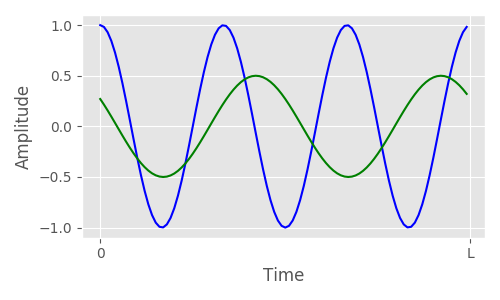
\includegraphics[scale = 0.8]{twoSinusoids.png}
	\label{fig:twoSines}
\end{figure}

Consider the two sinusoids in Figure 1, which will serve as a good example for illustrating orthogonality.  To 
take the inner product of these two sinusoids over some interval from 0 to some farther point in time $L$, 
one must sum the pointwise products of the amplitudes
for every instant in time between 0 and $L$.  The first pointwise product would be at $t = 0$ where $t$ 
represents time.  At that moment, the green sinusoid has an amplitude of about 0.25 and the blue sinusoid has
an amplitude of 1.0.  The product of these two values would be $1.0 * 0.25 = 0.25$.  That constitutes the first pointwise product.
To calculate the sum of all the other pointwise products, we would need to do this same procedure for every value of $t$
between 0 and $L$.  That's an infinite number of points!  Fortunately, 
if we can express these sinusoids in the form $A\sin(2\pi ft + \phi)$, then
it becomes relatively trivial with calculus and we can show that the result is indeed 0! 

Any two sinusoids of different frequencies are orthogonal no matter their phase or amplitude.  A key caveat though
is that the duration over which we take the inner product must usually be infinite in order to make this claim.  In 
music though, we never deal with infinitely long sine waves.  Songs are made up of finite length sine waves.  We
can still have orthogonality for any two sine waves over some finite interval from 0 to $L$, but we must provide
the extra condition that the waves are \textbf{periodic} along that interval.  This is a crucial point and one that 
will be paramount for 
understanding the limitations of the Discrete Fourier Transform.  If we look back at Figure \ref{fig:twoSines}, 
we will see that 
both the blue and the green sinusoids start and end at the same place in their respective curve.  If this were not true,
we could \textbf{not} make the claim that these two sine waves were orthogonal along that interval.  

Two periodic sinusoids are also orthogonal even when we sample them.  This is important because we will
never deal with periodic continuous sinusoids in a computer like those found in Figure \ref{fig:twoSines}.  We will be 
dealing with sampled signals and sinusoids.  To illustrate and provide a little proof on concept, let's sample the
two sinusoids from Figure \ref{fig:twoSines}.  For ease, let's assume that $L = 1$ so we will sample for one second
from both the green and blue sinusoids.  If you look at Figure \ref{fig:twoSines}, we can see that the green sinusoid
completes two complete cycles over a period of 1 second.  Therefore, it has a frequency of 2Hz.  The blue sinusoid
completes three full cycles so it has a frequency of 3Hz.  We need to choose a sampling rate that will not cause aliasing
for these two signals.  Anything above 6Hz will suffice, so let's choose 8 Hz.  Figure \ref{fig:twoSinesPoints} shows 
where those samples lie on our two sinusoids.  The samples for the blue sinusoid are approximately $b[n] = [1, -0.707, 0, 0.707, -1, 0.707, 0, -0.707]$ and the samples for the green
sinusoid are $g[n] = [0.27, -0.421, -0.27, 0.421, 0.27, -0.421, -0.27, 0.421]$.  The inner
product of $b[n]$ and $g[n]$ is equal to (1 * 0.27) + (-0.707 * -0.421) + (0 * -0.27) + 
(0.707 * 0.421) + (-1 * 0.27) + (0.707 * -0.421) + (0 * -0.27) + (-0.707 * 0.421) = 0.
Indeed these two sinusoids are orthogonal even when sampled.

\begin{figure}[h]
	\caption{Two sinusoids that are periodic along the interval 0 to $L$.}
	\centering
	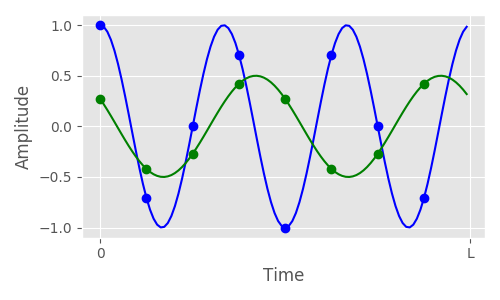
\includegraphics[scale = 0.8]{twoSinusoidsPoints.png}
	\label{fig:twoSinesPoints}
\end{figure}

Let's briefly summarize the conditions when two sinusoids of different frequencies
are orthogonal:

\begin{itemize}
	\item the two sinusoids are periodic along some time interval
	\item if sampled, the sample rate is greater than twice the frequency of both sinusoids
\end{itemize}

If you are curious more about how we can prove orthogonality and some of the issues with orthogonality for
continuous and discrete sinusoids, refer to Appendix A.

\section*{Probing for Sinusoids}

Ideally we would like some tool to be able to test whether a particular frequency is part
of some arbitrary signal.  We should be able to provide this tool some signal like a song
or speech and some frequency and our tool should be able to report back to use that either,
yes, this frequency is part of the signal or, no, the frequency is not part of the signal.
Figure \ref{fig:test} graphically depicts this procedure.  	Given such a tool, we could then 
iteratively test our signal for a whole range of frequencies
to construct the frequency domain of our signal.  This is exactly the procedure that the 
DFT performs.  It tests a signal for a whole range of frequencies to determine which are 
part of the signal and which are not.

\begin{figure}[h]
\caption{A sketch of the desired procedure for determining frequency in a signal.}
\centering
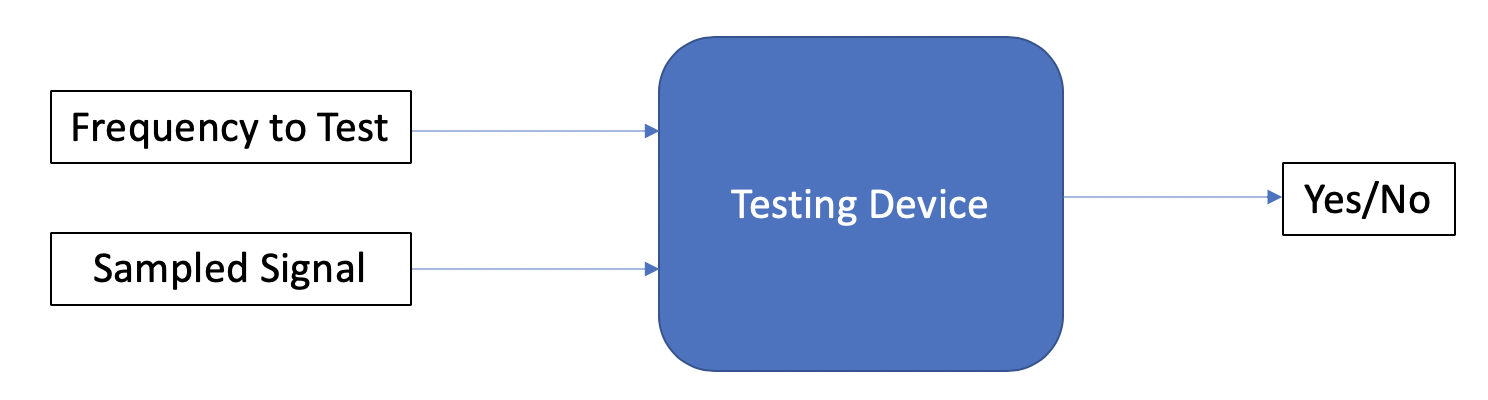
\includegraphics[scale = 0.4]{test.png}
\label{fig:test}
\end{figure}

Orthogonality will be our testing tool.  Let's imagine that our sampled signal was a simple
sinusoid of arbitrary frequency, phase, and amplitude.  Ahead of time, we do not know
anything about the sinusoid other than it is periodic along some time interval $L$.  Let's 
choose a frequency to test, say 100Hz, that we know is also periodic along $L$.  If we take
the inner product between the samples of the unknown sinusoid and the samples of 100Hz,
the result can provide some clues as to whether they are the same signal.  What do we know 
if the result is non-zero?  We can definitively conclude that they are the same frequency because
all periodic sinusoids of different frequencies are orthogonal.  What do we know if the result is 
zero?  The easy conclusion is to say that they must be different frequencies.  But that would
be a mistake!  We have not said anything yet about the inner product of two sinusoids of the
\textbf{same} frequency.  As it turns out, the inner product will almost always be non-zero 
unless the two sinusoids are out of phase by $\pi/2$.  So an inner product of zero almost
always means that the two sinusoids are of different frequency but not definitively.

	The inner product then is almost the perfect tool to help us distinguish between two
periodic frequencies.  Unfortunately, the pesky phase issue of $\pi/2$ for two sinusoids of 
the same frequency throws a wrench into the system.  In the next section, we will look at a way
to correct this problem.  But for now, let's assume that the inner product can perfectly distinguish
between the frequencies of two sinusoids.  

	We have shown how orthogonality can work as our testing tool for Figure \ref{fig:test} when
our signal is a sinusoid.  But rarely would our signal ever be just a simple sinusoid.  How can
we apply the inner product to an arbitrary signal like a song?  Recall that
any song, speech, soundscape, or any other kind of audio can be broken down into a sum of sinusoids.

$$A_1\sin(2\pi f_1 t + \phi_1) + A_2\sin(2 \pi f_2 t + \phi_2) + A_3\sin(2 \pi f_3 t + \phi_3) + ...$$

It turns out that the inner product is distributive.  So the inner product of some arbitrary signal applies
to each sinusoidal element that composes the signal.  The term ``distributive" in mathematics applies
to many different operations.  For example, we know from alebgra that the distributive property of 
multiplication over addition means that $x * (y + z) = x * y + x * z$.  We see that the multiplication operator can apply
to each individual component and the result is just the same.  If we have an arbitrary signal $x$ and another
arbitrary signal composed of components $y$ and $z$, then the distributive property for inner products 
means that  $\langle x, y + z \rangle = \langle x, y \rangle + \langle x, z \rangle$.  We will not spend any
time proving this truth here.  But it is actually not too difficult to do so.  The inner product is simply a
series of multiplications and additions.  So with some clever rearranging of terms, we can show that 
the distributive property is true for inner products.  

This is a wonderful result because we know now that when the inner product of some test frequency is 
applied to some arbitrary signal composed of sinusoids, the result is equivalent to the inner product of
our test frequency with each sinusoidal component.  We just analyzed the meaning of the inner product
of two sinusoids.  Anything that is non-zero means that two sinusoids are the same frequency.  Anything
zero is \textbf{almost} always means the two sinusoids are of different frequency.  Therefore, a non-zero result
of the inner product of some test frequency with an arbitrary signal means that the frequency is a part of that
signal.  A result of zero means that the frequency is likely not a part of the signal.  So the inner product
is our tool to implement Figure \ref{fig:test}.  

\begin{figure}[h]
	\caption{A realization of the desired procedure for determining frequency in a signal.}
	\centering
	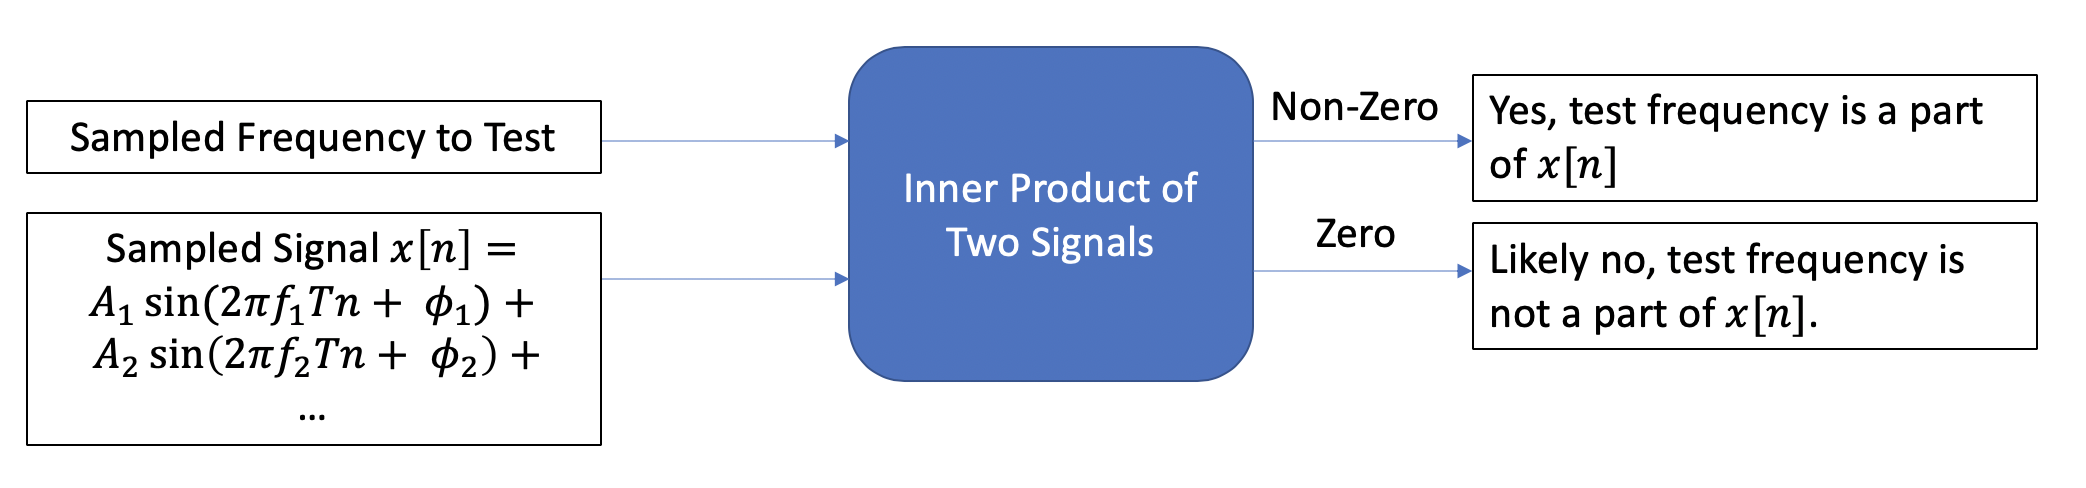
\includegraphics[scale = 0.4]{testImplemented.png}
	\label{fig:testImplemented}
\end{figure}

Figure \ref{fig:testImplemented} summarizes our methodology for implementing Figure \ref{fig:test}.  The inner
product is a tool that can distinguish whether two sinusoids are the same frequency with near certainty.  The next
section will show a way to make it foolproof.  Because the inner product is distributive, when it is applied to an
arbitrary signal and some test sinusoid, the inner product of the test with each sinusoidal component of different
frequency will be zero.  If any of the frequency components match our test frequency,  we will likely get a non-zero
result indicating that the test frequency is present in our signal.  Again, our test mechanism depicted in 
Figure \ref{fig:testImplemented} only works under the condition that the test frequency and the sampled signal
are periodic along the same interval.  

\section*{The Pesky $\pi/2$ Problem}

We know that the inner product of two sinusoids at different frequencies is always zero, assuming that the
sinusoids are periodic over some interval $L$.  However, that is not the $\textbf{only}$ way two sinusoids are
orthogonal.  It turns out that the inner product of two sinusoids of the $\textbf{same}$ frequency is zero when 
the sinusoids are separated by a phase of $\pi/2$.  This is a problem if we want to use the inner product to
test the similarity of two frequencies.  We do not want the inner product to be zero when the frequencies are the
same.  That should be reserved for different frequencies. 

How can we ensure that we get a non-zero inner product for sinusoids of the same frequency?  The answer:
take \textbf{two} inner products.  Suppose we have some test frequency and some signal and we would like to 
know whether that test frequency is a part of the signal just as described in Figure \ref{fig:test}.  If we take
the inner product between the test frequency and the signal, we run the risk that the answer could be zero even
if the test frequency is a part of the signal.  But if we have two test sinusoids of the same frequency but with
different phases, then at least one of them will yield a non-zero inner product with the signal if the signal 
contains the frequency of the test sinusoid.  

It may not be readibly apparent why using two sinusoids makes any difference.  For simplicity, let us say the
two sinusoids are sine and cosine.  Sine and cosine are separated by a phase difference of $\pi/2$.  Can you
think of another sinusoid of the same frequency with a phase different of $\pi/2$ for \textbf{both} of them?
The answer is no.  A sinusoid that $\pi/2$ away from cosine is either a sine wave or $\pi$ radians away from
sine.  In either case, that sinusoid would have a non-zero inner product with sine.  Therefore, using two inner
products, one with sine and one with cosine, creates a wonderful system where a zero inner product from both
cosine and sine means the frequency is conclusively not a part of the signal.

\begin{figure}[h]
	\caption{Complete solution for testing frequency components of a signal.}
	\centering
	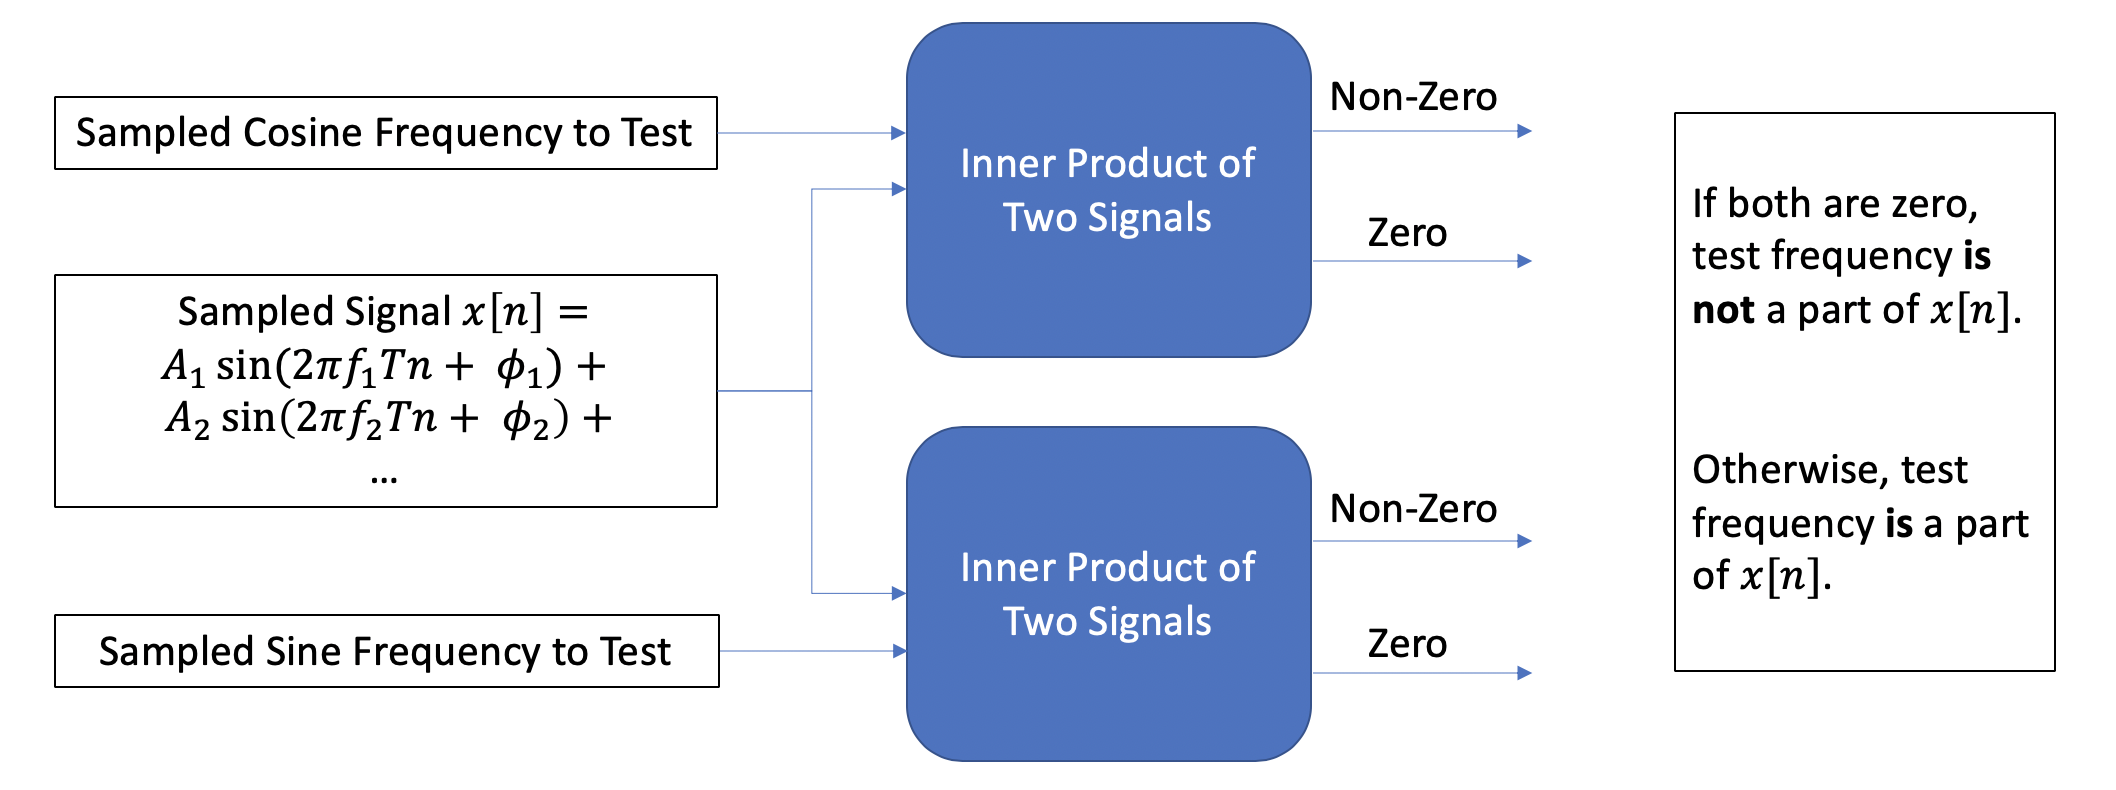
\includegraphics[scale = 0.4]{testComplete.png}
	\label{fig:testComplete}
\end{figure}

Figure \ref{fig:testComplete} shows our completed implementation of the testing mechanism outlined from
Figure \ref{fig:test}.  Note how we now need two sampled sinusoids: one cosine and one sine.  But now see
how an inner product of zero for both the sine test and cosine test definitively concludes that the frequency
is not a part of the signal.

If you are curious about how we can prove that $\pi/2$ is an issue, see Appendix B which walks through the math.

\section*{Imaginary Numbers}

Figure \ref{fig:testComplete} shows how we need to take the inner product of our signal with both a cosine and
sine wave to test whether a frequency is present in some signal.  Therefore, we will have two results, one for
each inner product.  It's a little cumbersome in math to express two separate results from some operation.  
Generally, if we compute something like $\sin(\pi/2)$, it yields a single numerical result.  

One way to do this would be to use vectors.  As we discussed above, vectors store a sequence of data and we
could put the result from the first inner product in the first slot of the vector and the second inner product in 
the second slot.  This would work perfectly well.  But there actually is a better solution: complex numbers.
Perhaps you have encountered complex numbers somewhere in your mathematical training.  Complex numbers
come in the form $a + bi$ where $i$ is called the imaginary unit or number and is defined as $i^2 = -1$.  Already,
this feels perilous on some level.  Why are we using complex numbers for audio signals?  There is nothing
``imaginary" about an audio signal, sine wave, or cosine wave.  So why use them?

In general, complex numbers are important mathematical tools for solving problems in mathematics, engineering and
the physical sciences.  This includes signals.  In fact, complex numbers are just as ``real" as say negative numbers.
It's hard to find a physical analogy to negative numbers.  We cannot pick up -4 rocks, for example.  Yet, we 
accept negative numbers because they allow us to work more easily with operators like subtraction.  Complex
numbers are similar.  They are a mathematical tool that allows us to solve problems we would not otherwise be
able to solve.  For our purposes, they serve a similar role to vectors.  When we have a number like $a + bi$, we
separate the real component $a$ from the imaginary component $b$.  You cannot add $a$ and $b$.  They are treated
as separate and distinct units.  We could very well use a complex number to express the number of apples and 
oranges.  Perhaps the real component represents the number of apples and the imaginary component represents
the number of oranges.  Then, to express that I have 3 apples and 4 oranges, I could write that as a single number
$3 + 4i$.  So one way to view a complex number is simply as a single number that has two distinct parts.  This
is what we need.  We can use the real component to hold the result of one inner product and the complex 
component to hold the other.

Complex numbers have one final important property that make them the ideal choice for our problem.  The great 
mathematician, Leonhard Euler, discovered one of the fundamental mathematical equations
that relates numbers such as $i$, $e$ and $\sin$ and $\cos$.  It is called Euler's formula:

\begin{equation}
\label{eq:euler}
e^{ix} = \cos(x) + i\sin(x)
\end{equation}

This is one of the most remarkable equations in all of mathematics.  The key takeaway is that we can use
a complex exponential to express both a real cosine term and an imaginary sine term.  Again there is
nothing ``imaginary" about the sine wave.  The complex exponential can simply be expressed as two 
\textbf{separate} sinusoids.  Fortuitously, a complex exponential is just what we need for our current
problem.  Remember we want to take the inner product of a signal with a cosine and sine wave, and we want to 
keep the results separate.  All we need to do then is to take the inner product of our signal with a complex
exponential.  For example, if we have a signal $x[n]$ and
we want to test it for frequency $f_{test}$, we can compute $\langle x[n], e^{2\pi f_{test}i}\rangle$.  This
notation says to take the inner product with the real cosine term of frequency $f_{test}$ and the inner
product with imaginary sine term of frequency $f_{test}$.  Because the real and imaginary numbers are kept
separate, we will get an answer of the form $a + bi$ where $a$ is the result of the inner product with cosine
and $b$ is the result of the inner product with sine. 

For digital signal processing, we will sometimes see Euler's formula express with a different variable $\omega$ which
stands for angular frequency.  Angular frequency is related to frequency by the equation $\omega = 2\pi f$.  So
we can rewrite Equation \ref{eq:euler} as $e^{i\omega} = \cos(\omega) + i\sin(\omega)$ or 
$e^{2\pi fi} = \cos(2 \pi f) + i\sin(2\pi f)$.  This better expresses the relationship between the frequency of the
sinusoids and the complex exponential.

Figure \ref{fig:testComplex} shows the updated version of our procedure for calculating the inner product.

\begin{figure}[h]
	\caption{Complete solution using complex exponentials.}
	\centering
	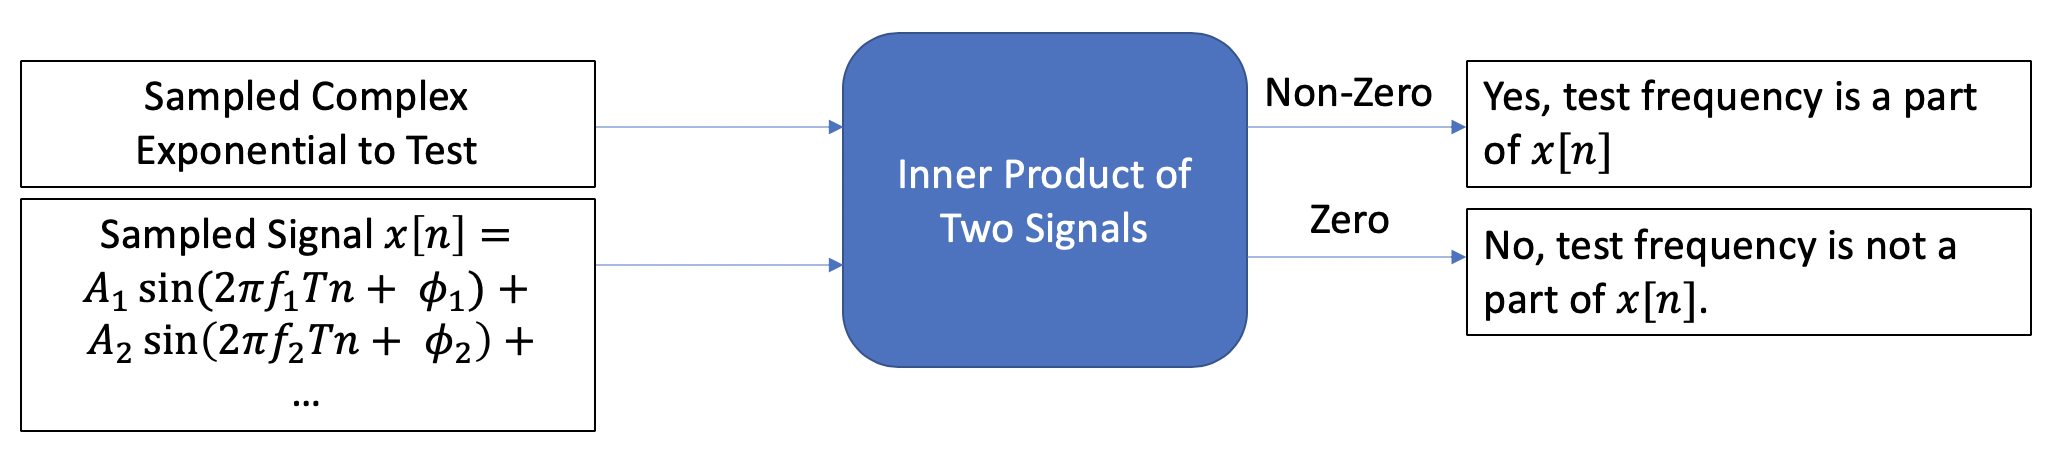
\includegraphics[scale = 0.4]{testComplex.png}
	\label{fig:testComplex}
\end{figure}

It is important to understand that Figure \ref{fig:testComplex} is no different from Figure \ref{fig:testComplete}.  
The inner product in Figure \ref{fig:testComplex} produces two inner products stored in the real and imaginary
components, respectively.  Those are the same inner products calculated in Figure \ref{fig:testComplete}.  If
both the real and imaginary component are zero then we know the test frequency is not a part of our signal
$x[n]$.

Unrelated to the issue of inner products, Euler's
formula also allows us to translate back and forth between sinusoids like sine and cosine and exponentials.
Exponentials are much easier to work with and allows us to quickly prove equations like trigonometric identities
that would be much harder if we simply had to work with just sine and cosine.  In general, if you plan to learn
more about digital signal processing, you will need to get comfortable with complex exponentials.

\textbf{**NEED TO MENTION ABOUT NEGATIVE AND SAY -SIN**}